\documentclass[titlepage = firstcover]{scrartcl}
\usepackage[aux]{rerunfilecheck}
\usepackage{fontspec}
\usepackage[main=ngerman, english, french]{babel}

% mehr Pakete hier
\usepackage{expl3}
\usepackage{xparse}

%Mathematik------------------------------------------------------
\usepackage{amsmath}   % unverzichtbare Mathe-Befehle
\usepackage{amssymb}   % viele Mathe-Symbole
\usepackage{mathtools} % Erweiterungen für amsmath
\usepackage[
  math-style=ISO,    % \
  bold-style=ISO,    % |
  sans-style=italic, % | ISO-Standard folgen
  nabla=upright,     % |
  partial=upright,   % /
]{unicode-math}% "Does exactly what it says on the tin."
\usepackage[section, below]{placeins}

% Laden von OTF-Mathefonts
% Ermöglich Unicode Eingabe von Zeichen: α statt \alpha

\setmathfont{Latin Modern Math}
%\setmathfont{Tex Gyre Pagella Math} % alternativ zu Latin Modern Math
\setmathfont{XITS Math}[range={scr, bfscr}]
\setmathfont{XITS Math}[range={cal, bfcal}, StylisticSet=1]

\AtBeginDocument{ % wird bei \begin{document}
  % werden sonst wieder von unicode-math überschrieben
  \RenewDocumentCommand \Re {} {\operatorname{Re}}
  \RenewDocumentCommand \Im {} {\operatorname{Im}}
}
\usepackage{mleftright}
\setlength{\delimitershortfall}{-1sp}

%Sprache----------------------------------------------------------
\usepackage{microtype}
\usepackage{xfrac}
\usepackage[autostyle]{csquotes}    % babel
\usepackage[unicode, pdfusetitle]{hyperref}
\usepackage{bookmark}
\usepackage[shortcuts]{extdash}
%Einstellungen hier, z.B. Fonts
\usepackage{booktabs} % Tabellen


\title{Gekoppelte elektrische Schwingungen}
\author{
  David Gutnikov\\
  \href{mailto:david.gutnikov@udo.edu}{david.gutnikov@udo.edu}
 \and 
  Lasse Sternemann\\
  \href{mailto:lasse.sternemann@udo.edu}{lasse.sternemann@udo.edu}
}
\date{Durchführung am 14.01.2020}


\begin{document}
  \maketitle
  \newpage
  \tableofcontents
  \newpage


\section{Zielsetzung}
    In diesem Versuch soll das Verhalten von gekoppelten Schwingkreisen genauer untersucht werden. Dazu werden nun elektrische Schwingkreise genutzt, da 
    deren Verhalten weitaus besser zu messen ist, als das eines mechanischen Schwingungssystems.
    
\section{Theorie}   
    \subsection{Kapazitiv gekoppelte Schwingkreise}
        \begin{figure}[h]
          \centering
          \caption{Das Schaltbild zur Erzeugung einer kapazitiv gekoppelten Schwingung. [1]}
          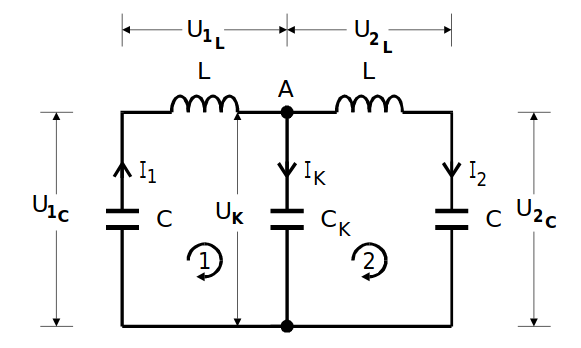
\includegraphics[width = 0.4\linewidth]{Schwingkreis.png}
          \label{fig:Schwingkreis}
        \end{figure}
        Ein kapazitiv gekoppelter Schwingkreis besteht aus zwei einzelnen Schwingkreisen, die über einen Kondensator gekoppelt sind. In diesem Versuch 
        werden dazu zwei LC-Schwingkreise verwendet, die wie in Abbildung \ref{fig:Schwingkreis} zu sehen geschaltet sind. Die Spulen haben hierbei dieselben Induktivitäten 
        und auch die Kapazitäten des linken und rechten Kondensators gleichen sich. Um nun die Differentialgleichungen des Systems zu bestimmen, müssen 
        zunächst die Zeitabhängigkeiten der Ströme und Spannungen betrachtet werden. Eine allgemeine Betrachtung der Ströme, über die kirchhoffsche 
        Knotenregel, in Punkt A ergibt für die Ströme:
        \begin{equation}
            I_1 = I_k + I_2 \qquad \Rightarrow \qquad I_k = I_1 - I_2
            \label{eqn:Knoten}
        \end{equation} 
        Die allgemeine Betrachtung der Spannungen in den Maschen 1 und 2 über die Kirchhoffsche Maschenregel liefert für beide Maschen:
        \begin{align*}
            U_\text{C} + U_\text{L} U_\text{K} = 0
        \end{align*}
        Durch Einsetzen der Zusammenhänge
        \begin{align*}
            U_{\text{C}} &= \frac{1}{\text{C}} \int I dt\\
            U_{\text{L}} &= \text{L} \cdot \dot{I}
        \end{align*}
        und unter Berücksichtigung von Beziehung \ref{eqn:Knoten} ergibt sich nach einer zeitlichen Ableitung pro Schwingkreis eine Differentialgleichung.
        \begin{align}
            \text{Schwingkreis 1:} \qquad L\ddot{I_1} + \frac{I_1}{C} + \frac{\left(I_1 - I_2\right)}{C_k} = 0 \\
            \text{Schwingkreis 2:} \qquad L\ddot{I_2} + \frac{I_2}{C} - \frac{\left(I_1 - I_2\right)}{C_k} = 0 
            \label{eqn:ProtoDGL}
        \end{align}
        Um homogene Differentialgleichungen zu erhalten werden nun die Differenz oder Summe der Ströme $I_1$ und $I_2$ betrachtet. Dies gelingt durch 
        einfaches Addieren bzw. Subtrahieren der beiden Gleichungen \ref{eqn:ProtoDGL}. 
        Die sich dadurch ergebenden homogenen Differentialgleichungen
        \begin{align}
            \text{Stromsumme} &: \qquad L \cdot \frac{d²}{dt²}\left(I_1+I_2\right) + \frac{1}{C} \cdot \left(I_1 + I_2\right) = 0 \\
            \text{Stromdifferenz} &: \qquad L \cdot \frac{d²}{dt²}\left(I_1-I_2\right) + \left(\frac{1}{C}+\frac{2}{C_k}\right) \cdot \left(I_1 - I_2\right) = 0
        \end{align}
        Die Lösung zur Differentialgleichung der Stromsumme entspricht einer harmonischen Schwingung mit der Schwingungsfrequenz:
        \begin{equation}
            \left(I_1 + I_2\right)(t) = \left(I_{1,0} + I_{2,0}\right) \cdot cos(\frac{t}{\sqrt{\text{LC}}}) \\
            \nu^+ = (2\pi \cdot \sqrt{\text{LC}})^{-1} 
            \label{eqn:nu+}
        \end{equation}
        Diese Schwingungsfrequenz entspricht der eines einzelnen LC-Kreises und die Amplitude der Stromsumme entspricht der Summe der einzelnen 
        Stromamplituden. \newline
        Analog dazu schwingt die Lösung der Stromdifferenz mit der Differenz der einzelnen Stromamplituden und mit folgender Frequenz:
        \begin{align}
            \left(I_1 - I_2\right)(t) &= \left(I_{1,0} - I_{2,0}\right) \cdot cos\left[\frac{t}{\sqrt{\text{L} \cdot \left(\frac{1}{C}+\frac{2}{C_k}\right)^{-1}}}\right] \\
            \nu^- &= \left[2pi \cdot \sqrt{L \cdot \left(\frac{1}{C}+\frac{2}{C_k}\right)^{-1}}\right]^{-1} 
            \label{eqn:nu-}
        \end{align}
        Um nun die eigentlich gesuchten Funktionen der einzelnen Ströme zu erhalten, muss der vorherige Trick wieder rückgängig, gemacht werden, also 
        die Lösungen der Schwingungen addiert bzw. subtrahiert werden, sodass sich die Lösungen für die einzelnen Ströme ergeben.
        \begin{align}
            I_1(t) = \frac{1}{2}(I_{1,0}+I_{2,0}) \cdot cos(2\pi \nu^+t) + \frac{1}{2}(I_{1,0}-I_{2,0}) \cdot cos(2\pi \nu^-t) \\
            I_2(t) = \frac{1}{2}(I_{1,0}+I_{2,0}) \cdot cos(2\pi \nu^+t) - \frac{1}{2}(I_{1,0}-I_{2,0}) \cdot cos(2\pi \nu^-t) 
            \label{eqn:EinzelDGL}
        \end{align}
        Eine Betrachtung dieser beiden Differentialgleichungen lässt auf zwei Spezialfälle schließen. Der eine ergibt sich, wenn beide Anfangsamplituden gleich
        sind. In diesem Fall verschwindet die zweite Fundamentalschwingung nämlich komplett und nur der $\nu⁺$-Anteil schwingt. Andersherum verschwindet der
        $\nu⁺$-Anteil und die erste Fundamentalschwingung, wenn die Anfangsamplituden zwar betragsmäßig gleich sind, jedoch entgegengesetzte Vorzeichen haben.
        Abgesehen von diesen Fundamentalschwingungen kann es auch zu einer Schwebung kommen, wenn zu Beginn nur einer der Schwingkreise schwingt und die 
        Anfangsamplitude der anderen Schwingung demnach gleich null ist. Für diese Schwebungen ergben sich folgende Schwingungsgleichungen:
        \begin{align}
            I_1(t) &= I_{1,0} \cdot cos\left(\frac{1}{2}\left(\nu⁺ + \nu⁻\right)t\right) \cdot cos\left(\frac{1}{2}\left(\nu⁺ - \nu⁻\right)t\right) \qquad \text{bei} \; I_{2,0} = 0\\
            I_2(t) &= I_{1,0} \cdot sin\left(\frac{1}{2}\left(\nu⁺ + \nu⁻\right)t\right) \cdot sin\left(\frac{1}{2}\left(\nu⁺ - \nu⁻\right)t\right)
            \label{eqn:Schwebung}
        \end{align} 
        Bei der Schwebung ändert sich die Amplitude mit der Schwebungsfrequenz
        \begin{equation}
            \nu_{\text{Schwebung}} = \nu⁺ - \nu⁻ \\
            \label{eqn:Schwebungsfrequenz}
        \end{equation}
        während die eigentliche Schwingung mit der Schwingungsfrequenz
        \begin{equation}
            \nu_{\text{Schwingung}} = \frac{1}{2}(\nu⁺ - \nu⁻) \qquad \text{und bei nahezu gleicher Frequenz} \qquad \nu_{\text{Schwingung}} \approx \nu⁺ \\
            \label{eqn:SchwebungSchwingung}
        \end{equation}
        Der Unterschied zwischen diesen zwei Frequenzen ist in Abbildung \ref{fig:Schwebung} zu erkennen.
        \begin{figure}[h]
            \centering
            \caption{Das Schwingverhalten einer Schwebung in der die Schwebungsfrequenz (oben) und die eigentliche Frequenz der Schwingung (unten) zu sehen ist.[1]}
            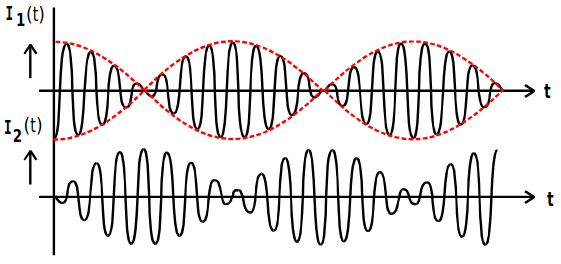
\includegraphics[width = 0.4\linewidth]{Schwebung.png}
            \label{fig:Schwebung}
        \end{figure}

    \subsection{Frequenzabhängigkeit des Stroms im kapazitiv gekoppelten Schwingkreis}
        \begin{figure}[h]
            \centering
            \caption{Das Schaltbild des kapazitiv gekoppelten Schwingkreis bei äußerer Anregung durch einen Sinusgenerator. Die Widerstände stehen dabei für sämtliche in den Schwingkreisen auftretende Verluste. [1] }
            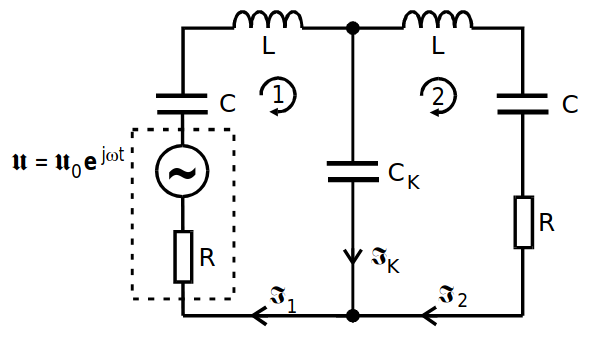
\includegraphics[width = 0.4\linewidth]{Strom.png}
            \label{fig:Strom}
        \end{figure}
        Für die in Abbildung \ref{fig:Strom} zu sehenden Maschen ergebn sich über die Kirchhoffsche Maschenregel folgende Terme:
        \begin{align}
            \text{Masche 1} &= (Z_C + Z_L + Z_{C_k} + Z_R) \cdot I_1 - Z_{C_k} \cdot I_2 = U \\
            \text{Masche 2} &= (Z_C + Z_L + Z_{C_k} + Z_R) \cdot I_2 - Z_{C_k} \cdot I_1 = 0 
            \label{eqn:Mascheangeregt}
        \end{align}
        Dabei stehen die Zs für die Impedanzen der Kondensatoren, Spulen und Widerstände.
        \begin{align*}
            Z_C = -j\frac{1}{\omega C} \qquad Z_L= j\omega L \qquad  Z_{C_k} = -j\frac{1}{\omega C_k} \qquad Z_R = R \\
        \end{align*}
        Durch Eliminieren von $I_1$ lässt sich aus \ref{eqn:Mascheangeregt} folgende Formel für den Betrag von $I_2$ herleiten:
        \begin{align}
            |I_2| = |U| \cdot \frac{1}{\sqrt{4\omega²C_k^2R²Z(\omega)²+\left(\frac{1}{\omega C_k}-\omega C_kZ(\omega)²+\omega R^2 C_k\right)²}} \\
            \text{mit} \qquad Z(\omega) = \omega L - \frac{1}{\omega}\left(\frac{1}{C} + \frac{1}{C_k}\right) 
            \label{eqn:Z(w)}
        \end{align} 
        Bei zwei Resonanzfrequenzen wird $I_2$ maximal. Die zugehörigen maximalen Ströme lassen sich wiefolgt berechnen:
        \begin{align}
            |I(\omega⁺)| = \frac{1}{R \cdot \sqrt{4 + \frac{R²C_k^2}{LC}}} \\
            |I(\omega⁻)| = \frac{1}{R \cdot \sqrt{4 + \frac{R²C_k^2}{LC} \cdot \left(1 + \frac{C}{C_k}\right)}} 
            \label{eqn:Resonanzstrom}
        \end{align}
        In der Praxis lassen sich beide Ströme durch 
        \begin{equation}
            |I(\omega⁺)| \approx |I(\omega⁻)| \approx \frac{1}{2R} \\
            \label{eqn:Näherung}
        \end{equation}
        annähern, da der restliche Teil der Wurzelterme vernachlässigbar klein ist.

\section{Durchführung}
    \subsection{Justierung}
        Gekoppelte Schwingungen basieren darauf, dass die einzelnen Schwinger untereinander Energie übetragen. Damit dieser Prozess vollständig ablaufen kann
        müssen die beiden Schwingkreise auf dieselbe Resonanzfrequenz justiert werden. Dazu wird zunächst über Schaltung \ref{fig:Justierung} die 
        Resonanzfrequenz des Schwingkreises mit fester Kapazität bestimmt. Dies geschieht indem die Phasenverschiebung zwischen Generatorspannung und 
        Schwingkreisstrom gemessen wird. Dazu werden die im XY-Betrieb entsstehenden Lissajous-Figuren verwendet, da sie verschwinden, wenn die 
        Resonanzfrequenz erreicht ist. Der andere Schwingkreis wird daraufhin mit derselben Schaltung auf die gemessene Resonanzfrequenz justiert, indem 
        dessen Kapazität variiert wird.
        \begin{figure}[h]
            \centering
            \caption{Das Schaltbild zur Justierung der beiden Schwingkreise.}
            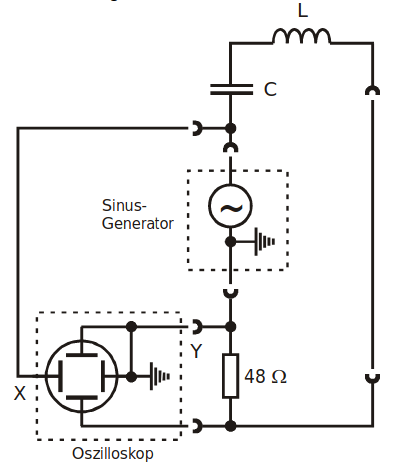
\includegraphics[width = 0.4\linewidth]{Justierung.png}
            \label{fig:Justierung}
          \end{figure}

    \subsection{Energieaustausch}
        Zunächst soll der Energieaustausch zwischen den beiden Schwingkreisen beobachtet werden. Hierfür wird einer der Schwingkreise durch ein Rechtecksignal
        extern angeregt und die Spannung des anderen, nicht angeregten Stromkreises am Oszilloskop dargestellt. Das zugehörige Schaltbild findet sich in 
        Abbildung \ref{fig:Energieaustausch}. Auf dem Oszilloskopbild kann die Schwebung direkt erkannt werden und das Verhältnis aus Schwebungs- und Schwingungsfrequenz ermittelt
        werden, indem die Maxima oder Minima der Schwingung innerhalb einer Schwebung abgezählt werden. Dieses Vorgehen wird für verschiedene Kapazitäten des
        Koppelkondensators $C_k$ wiederholt.
        \begin{figure}[h]
            \centering
            \caption{Das Schaltbild zur Beobachtung des Energieaustauschs zwischen den beiden Schwingkreisen.}
            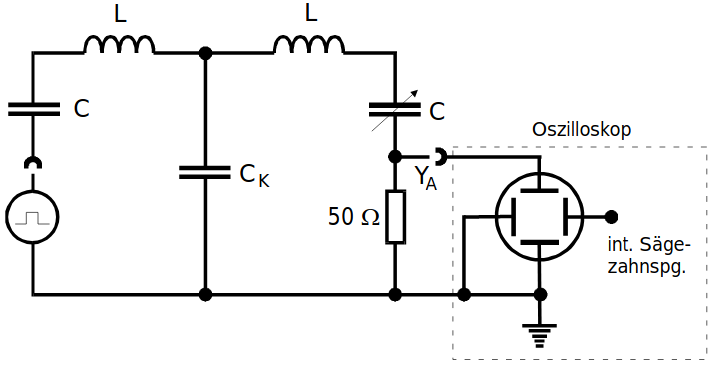
\includegraphics[width = 0.4\linewidth]{Energieaustausch.png}
            \label{fig:Energieaustausch}
          \end{figure}

    \subsection{Messung der Fundamentalfrequenzen}
          Nun sollen die Fundamentalfrequenzen in Abhängigkeit von verschiedenen Kapazitäten des Koppelkondensators $C_k$ gemessen werden. Dazu wird dieselbe Schaltung 
          genutzt mit dem Unterschied, dass über einen Sinusgenerator angeregt wird. Die Generatorspannung und die des nicht extern angeregten Schwingkreises werden
          werden im XX-Betrieb auf das Oszilloskop gegeben und die Frequenz wird wieder über Lissajous-Figuren ermittelt. Sie sind vorhanden, wenn eine 
          Phasenverschiebung von 0 (aufsteigende Gerade auf Oszilloskop) oder $\pi$ (absteigende Gerade auf Oszilloskop) vorliegt. 
          
    \subsection{Messung des frequenzabhängigen Stromverläufe}
          Um den Verlauf der Stomstärken zu messen wird eine Schaltung genutzt, die der in Abbildung \ref{fig:Stromverlauf} ähnelt. Der Unterschied liegt darin, dass kein 
          XY-Schreiber vorhanden ist und die Stromstärke daher anders bestimmt werden muss. Daher wird die an R abfallende Spannung  für beide 
          Fundamentalschwingungen über ein Oszilloskop gemessen. Dies erfolgt unter Variation der Kapazität des Koppelkondensators. Die Stromstärke wird 
          später über die gemessenen Spannungen und die Widerstände der Schaltung bestimmt. 
          \begin{figure}[h]
            \centering
            \caption{Das Schaltbild zur Beobachtung des Energieaustauschs zwischen den beiden Schwingkreisen.}
            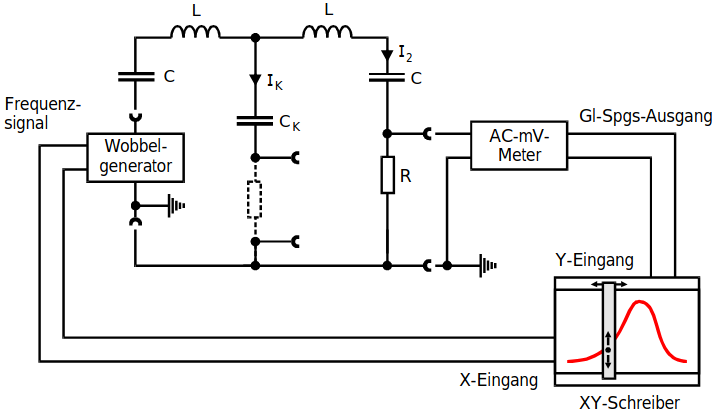
\includegraphics[width = 0.4\linewidth]{Stromverlauf.png}
            \label{fig:Stromverlauf}
          \end{figure}

\end{document}
          